\chapter{Appendix B - Hardware and Firmware}


\section{Schematics}

LearnAir V2 schematics are below.

\FloatBarrier

\begin{figure}[htb]
 	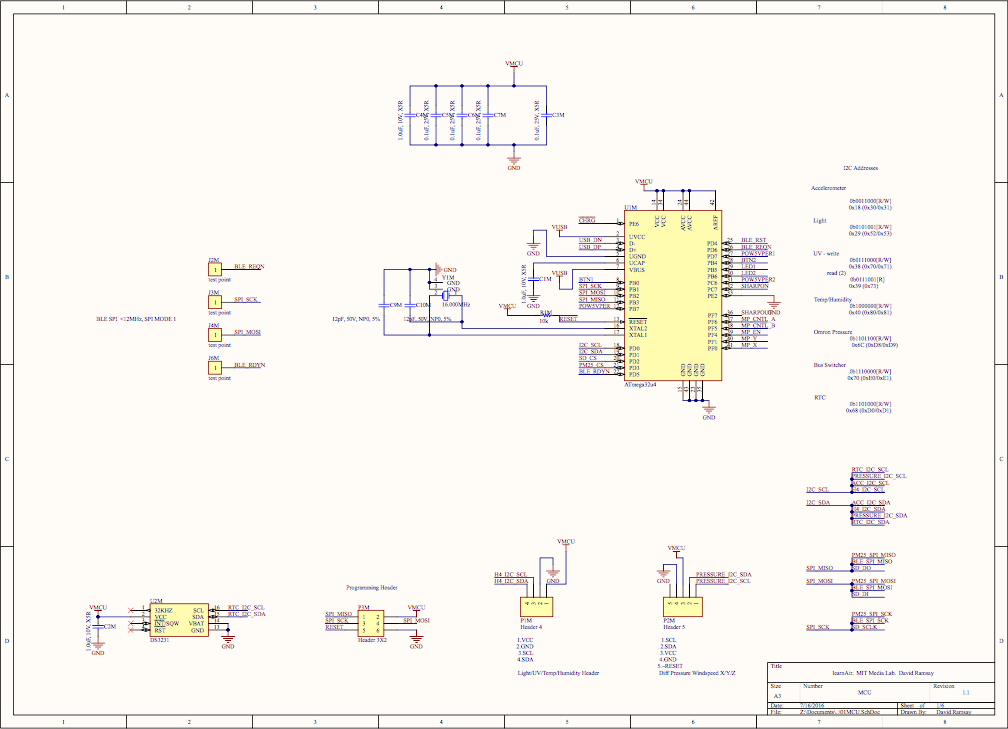
\includegraphics[width=\textwidth + \marginparwidth]{schematics/la_schematic1}               
\end{figure}
\begin{figure}[htb]
 	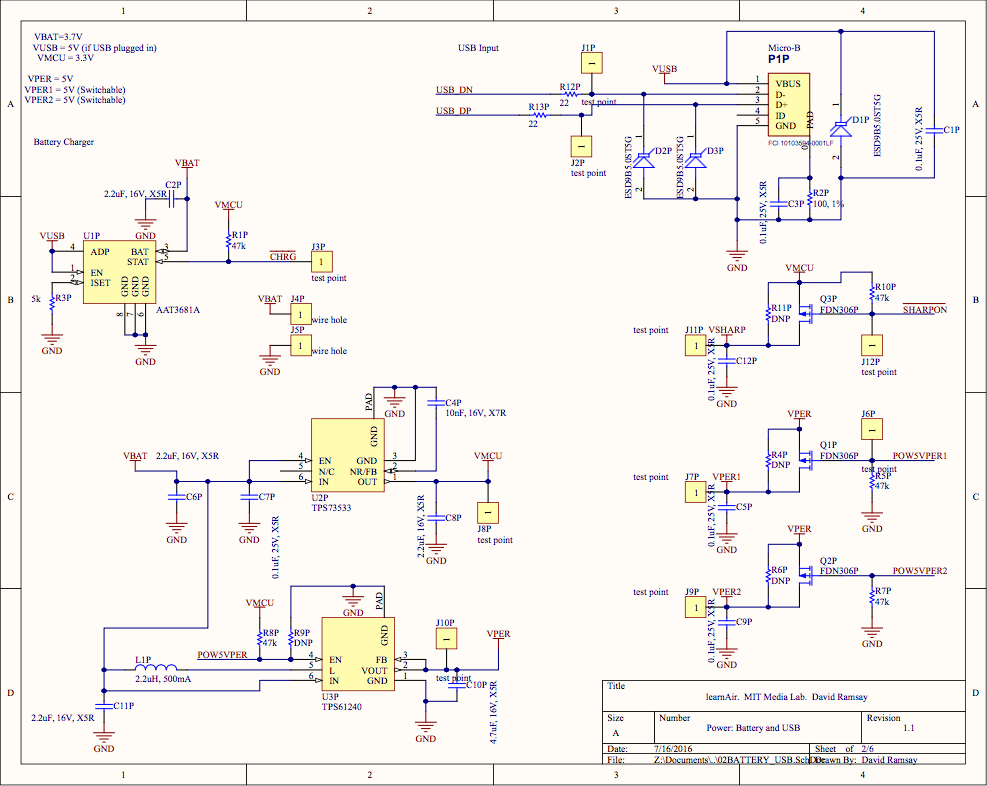
\includegraphics[width=\textwidth + \marginparwidth]{schematics/la_schematic2} 
 	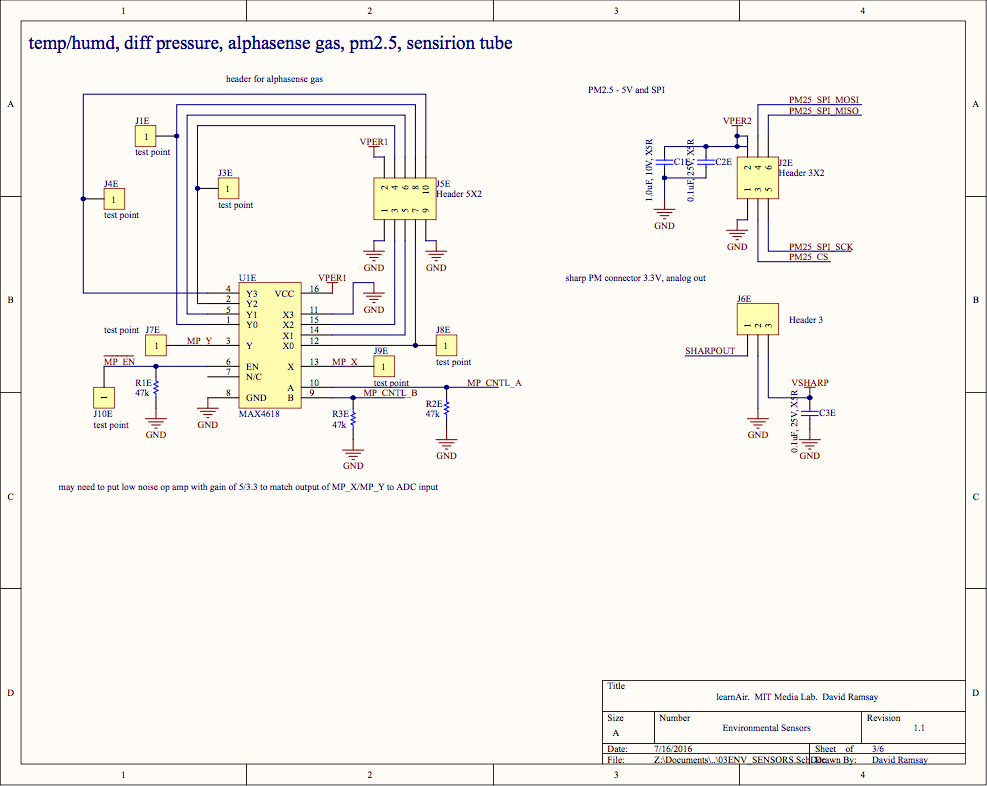
\includegraphics[width=\textwidth + \marginparwidth]{schematics/la_schematic3}                 
\end{figure}

\begin{figure}[htb]
 	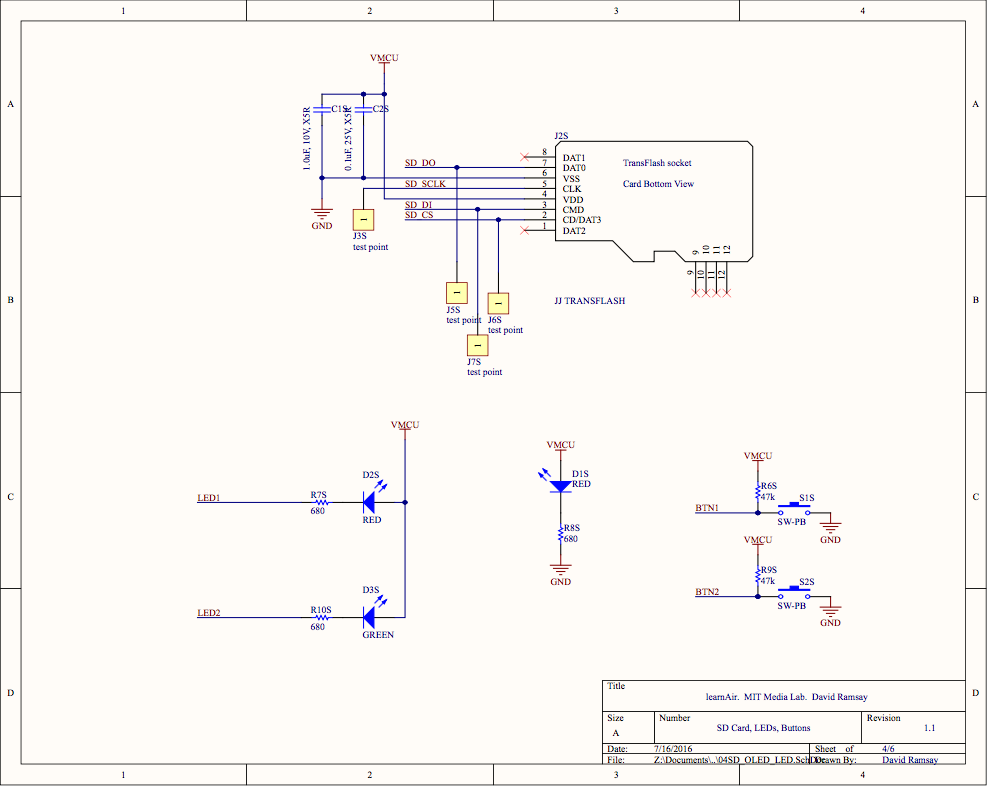
\includegraphics[width=\textwidth + \marginparwidth]{schematics/la_schematic4} 
 	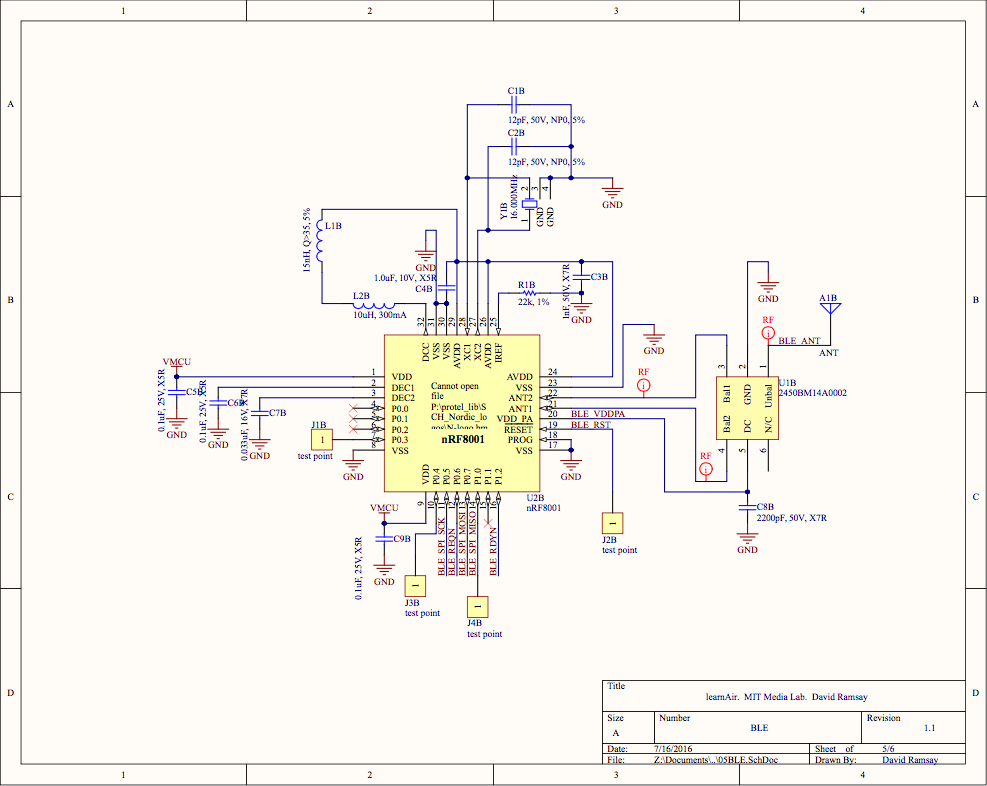
\includegraphics[width=\textwidth + \marginparwidth]{schematics/la_schematic5}              
\end{figure}
\begin{figure}[htb]
 	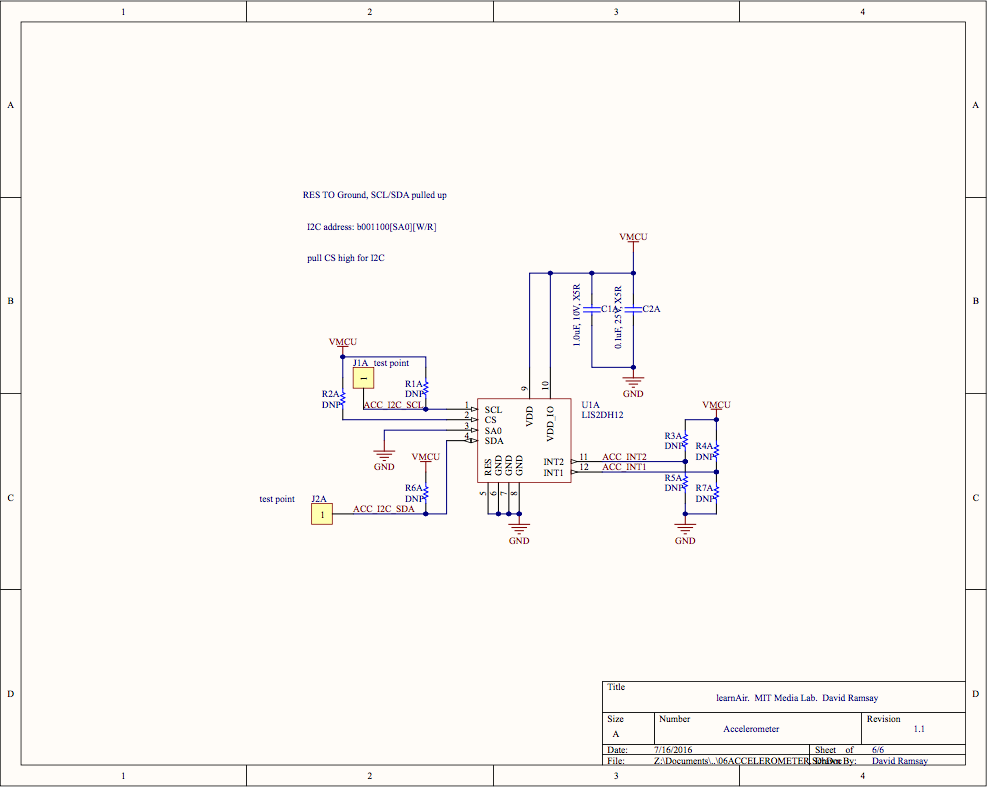
\includegraphics[width=\textwidth + \marginparwidth]{schematics/la_schematic6}               
\end{figure}

\FloatBarrier
LearnAir V3 uses the same schematics for peripherals, power, accelerometer, and BLE as for LearnAir V2.  The two differing schematics (MCU and SD Card) are shown below. 
\FloatBarrier

\begin{figure}[htb]
 	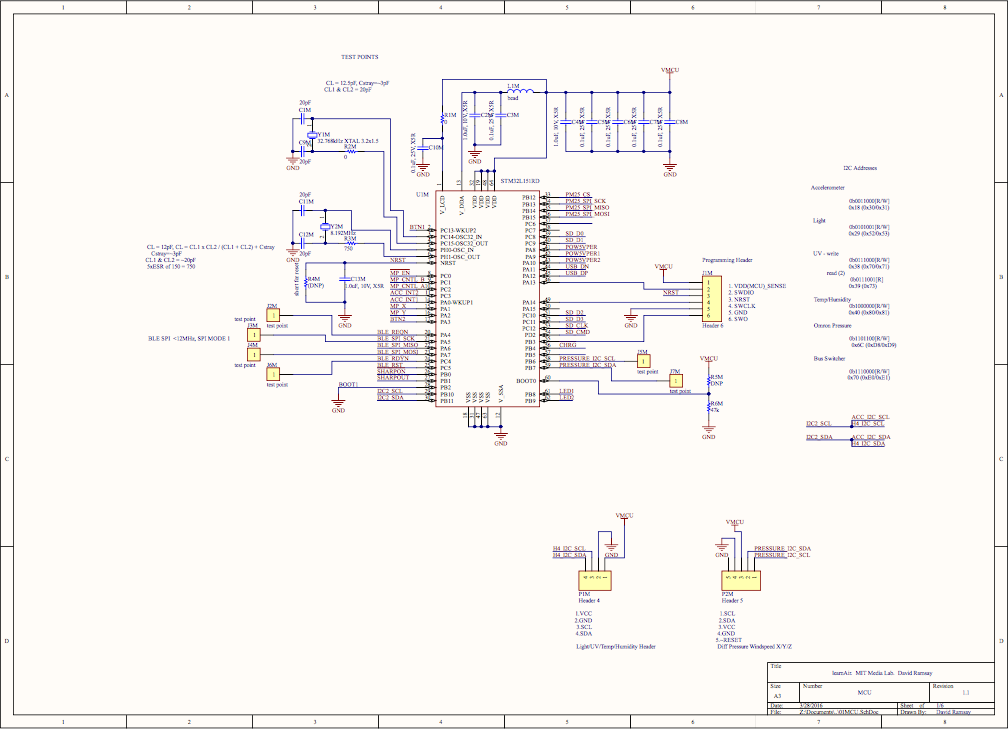
\includegraphics[width=\textwidth + \marginparwidth]{schematics/l3_schematic1}            
\end{figure}

\begin{figure}[htb]
	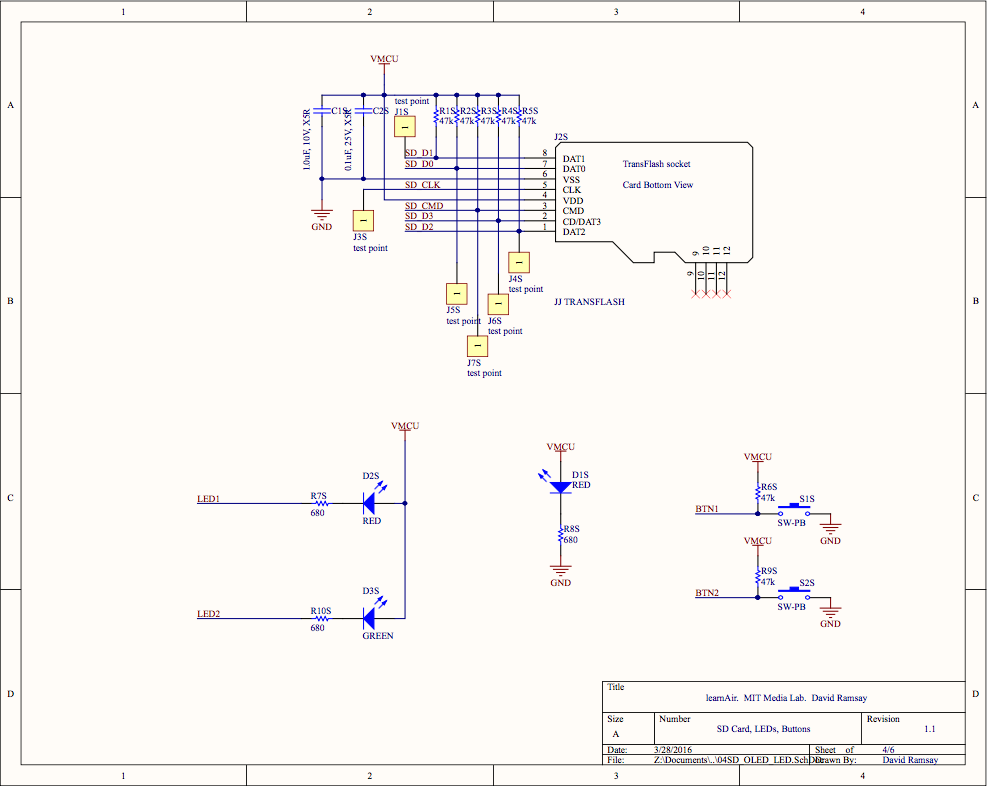
\includegraphics[width=\textwidth + \marginparwidth]{schematics/l3_schematic2}     
\end{figure}

\FloatBarrier
\section{Firmware}
\FloatBarrier

Below is the firmware for LearnAir V1.  Code written for LearnAir V2 and V3 is under development on github at \url{http://github.com/dramsay9/learnair}.

\begin{lstlisting}[style=code]
#include "RTClib.h"
#include "SD.h"
#include "SPI.h"
#include <Wire.h>

//RTC 
RTC_DS1307 RTC;
DateTime startTime;

//SD Card
File sensorData;

//Sharp Dust Sensor
int dustPin=0;
int dustVal=0;
int ledPower=11;
int delayTime=280;
int delayTime2=40;

//Pressure Sensor
unsigned int pressureVal = 0;

//Alphasense Sensor
int asensePin=1;
int asenseValS1W=0;
int asenseValS1A=0;
int asenseValS2W=0;
int asenseValS2A=0;
int asenseValS3W=0;
int asenseValS3A=0;
int asenseValTemp=0;
int aSelAPin=10;
int aSelBPin=9;
int aSelCPin=8;



void setup() {

  //RTC
  RTC.begin();
  
  if (! RTC.isrunning()) {
    RTC.adjust(DateTime(__DATE__, __TIME__)); 
  }
  
  //pressure I2C bus
  Wire.begin();
  Wire.beginTransmission(0x6C);
  Wire.write(byte(0x0B));
  Wire.write(byte(0x00));
  Wire.endTransmission();  
  
  Serial.begin(9600);
  
  
  
  //SD Card
  Serial.print("Initializing SD card...");
  // see if the card is present and can be initialized:
  if (!SD.begin(10, 11, 12, 13)) {
    Serial.println("Card failed, or not present");
    return;
  }

  //Create SD Card Title
  sensorData = SD.open("data.csv", FILE_WRITE);
  if (sensorData){
   sensorData.println("timestamp, alphaS1_work, alphaS1_aux, alphaS2_work, alphaS2_aux, alphaS3_work, alphaS3_aux, alphaTemp, sharpDust, pressureWind"); 
  }
  sensorData.close();
  
  Serial.println("card initialized.");

  //Sharp Dust Sensor
  pinMode(ledPower,OUTPUT);
  pinMode(4, OUTPUT);
  
  //Alphasense Sensor
  pinMode(aSelAPin, OUTPUT);
  pinMode(aSelBPin, OUTPUT);
  pinMode(aSelCPin, OUTPUT);

  delay(100);
  Serial.println("SETUP DONE. SENSOR READY.");

}



void loop() {
 
  //RTC Start
  startTime = RTC.now();
  
  sharpSense();
  pressureSense();
  alphaSense();
  
  //SD Write
  saveData(); 

  //Print Written Data
  printData();

  //Wait 30 seconds
  delay(30000); 

}


void saveData(){

  sensorData = SD.open("data.csv", FILE_WRITE);
  if (sensorData){
    
    sensorData.print(startTime.year(), DEC);
    sensorData.print('/');
    sensorData.print(startTime.month(), DEC);
    sensorData.print('/');
    sensorData.print(startTime.day(), DEC);
    sensorData.print(' ');
    sensorData.print(startTime.hour(), DEC);
    sensorData.print(':');
    sensorData.print(startTime.minute(), DEC);
    sensorData.print(':');
    sensorData.print(startTime.second(), DEC);
    sensorData.print(",");
    
    sensorData.print(asenseValS1W);
    sensorData.print(",");
    sensorData.print(asenseValS1A);
    sensorData.print(",");
    sensorData.print(asenseValS2W);
    sensorData.print(",");
    sensorData.print(asenseValS2A);
    sensorData.print(",");
    sensorData.print(asenseValS3W);
    sensorData.print(",");
    sensorData.print(asenseValS3A);
    sensorData.print(",");
    sensorData.print(asenseValTemp);
    sensorData.print(",");
    
    sensorData.print(dustVal);
    sensorData.print(",");
    sensorData.println(pressureVal);
    
    sensorData.close(); // close the file
    
    Serial.println("Wrote to file.");
  }
  else{
    Serial.println("Error writing to file!");
  }

}


void sharpSense(){
  
  digitalWrite(ledPower,LOW); // power on the LED
  delayMicroseconds(delayTime);
  dustVal=analogRead(dustPin); // read the dust value
  delayMicroseconds(delayTime2);
  digitalWrite(ledPower,HIGH); // turn the LED off

}


void pressureSense(){
  
  Wire.beginTransmission(0x6C);
  Wire.write(byte(0x00));
  Wire.write(byte(0xD0));
  Wire.write(byte(0x40));
  Wire.write(byte(0x18));
  Wire.write(byte(0x06));
  Wire.endTransmission();
  
  Wire.beginTransmission(0x6C);
  Wire.write(byte(0x00));
  Wire.write(byte(0xD0));
  Wire.write(byte(0x51));
  Wire.write(byte(0x2C));
  Wire.endTransmission();
  
  Wire.beginTransmission(0x6C);
  Wire.write(byte(0x07));
  Wire.endTransmission();

  Wire.requestFrom(0x6C, 2);    // request 2 bytes from Pressure Sensor

  if (2 <= Wire.available())  {  // if two bytes were received
    pressureVal = Wire.read();  // receive high byte (overwrites previous reading)
    pressureVal = pressureVal << 8;    // shift high byte to be high 8 bits
    pressureVal |= Wire.read(); // receive low byte as lower 8 bits
  }  
  
}


void alphaSense() {
  
  const int delayNum = 10;
  
  digitalWrite(aSelCPin,LOW);
  digitalWrite(aSelBPin,LOW);
  digitalWrite(aSelAPin,HIGH);
  delayMicroseconds(delayNum);
  asenseValS1W=analogRead(asensePin); 
  
  digitalWrite(aSelCPin,LOW);
  digitalWrite(aSelBPin,HIGH);
  digitalWrite(aSelAPin,LOW);
  delayMicroseconds(delayNum);
  asenseValS1A=analogRead(asensePin); 
  
  digitalWrite(aSelCPin,LOW);
  digitalWrite(aSelBPin,HIGH);
  digitalWrite(aSelAPin,HIGH);
  delayMicroseconds(delayNum);
  asenseValS2W=analogRead(asensePin); 
  
  digitalWrite(aSelCPin,HIGH);
  digitalWrite(aSelBPin,LOW);
  digitalWrite(aSelAPin,LOW);
  delayMicroseconds(delayNum);
  asenseValS2A=analogRead(asensePin); 
  
  digitalWrite(aSelCPin,HIGH);
  digitalWrite(aSelBPin,LOW);
  digitalWrite(aSelAPin,HIGH);
  delayMicroseconds(100);
  asenseValS3W=analogRead(asensePin); 
  
  digitalWrite(aSelCPin,HIGH);
  digitalWrite(aSelBPin,HIGH);
  digitalWrite(aSelAPin,LOW);
  delayMicroseconds(delayNum);
  asenseValS3A=analogRead(asensePin); 
    
  digitalWrite(aSelCPin,HIGH);
  digitalWrite(aSelBPin,HIGH);
  digitalWrite(aSelAPin,HIGH);
  delayMicroseconds(delayNum);
  asenseValTemp=analogRead(asensePin);
  
}


void printData(){
 
     
    Serial.print(startTime.year(), DEC);
    Serial.print('/');
    Serial.print(startTime.month(), DEC);
    Serial.print('/');
    Serial.print(startTime.day(), DEC);
    Serial.print(' ');
    Serial.print(startTime.hour(), DEC);
    Serial.print(':');
    Serial.print(startTime.minute(), DEC);
    Serial.print(':');
    Serial.print(startTime.second(), DEC);
    Serial.println("-------------------------------------");

    
    Serial.print("Alphasense Sensor 1.  Working: ");
    Serial.print(asenseValS1W);
    Serial.print("  Aux:  ");
    Serial.println(asenseValS1A);
    Serial.print("Alphasense Sensor 2.  Working: ");
    Serial.print(asenseValS2W);
    Serial.print("  Aux:  ");
    Serial.println(asenseValS2A);
    Serial.print("Alphasense Sensor 3.  Working: ");
    Serial.print(asenseValS3W);
    Serial.print("  Aux:  ");
    Serial.println(asenseValS3A);
    
    Serial.print("Alphasense Temp: ");
    Serial.println(asenseValTemp);
    
    Serial.print("Sharp Dust: ");
    Serial.println(dustVal);
    Serial.print("Pressure: ");
    Serial.println(pressureVal);
    
}
\end{lstlisting}

\FloatBarrier
\section{Hardware Analysis}
\FloatBarrier

Figure \ref{fig:ws_with_10_accuracy} shows the windspeed measurement comparison between our conditioned pressure sensor measurement and the MassDEP windspeed measurement. Within $\pm$5\% is denoted with green highlights.

\begin{figure}[htb]
 	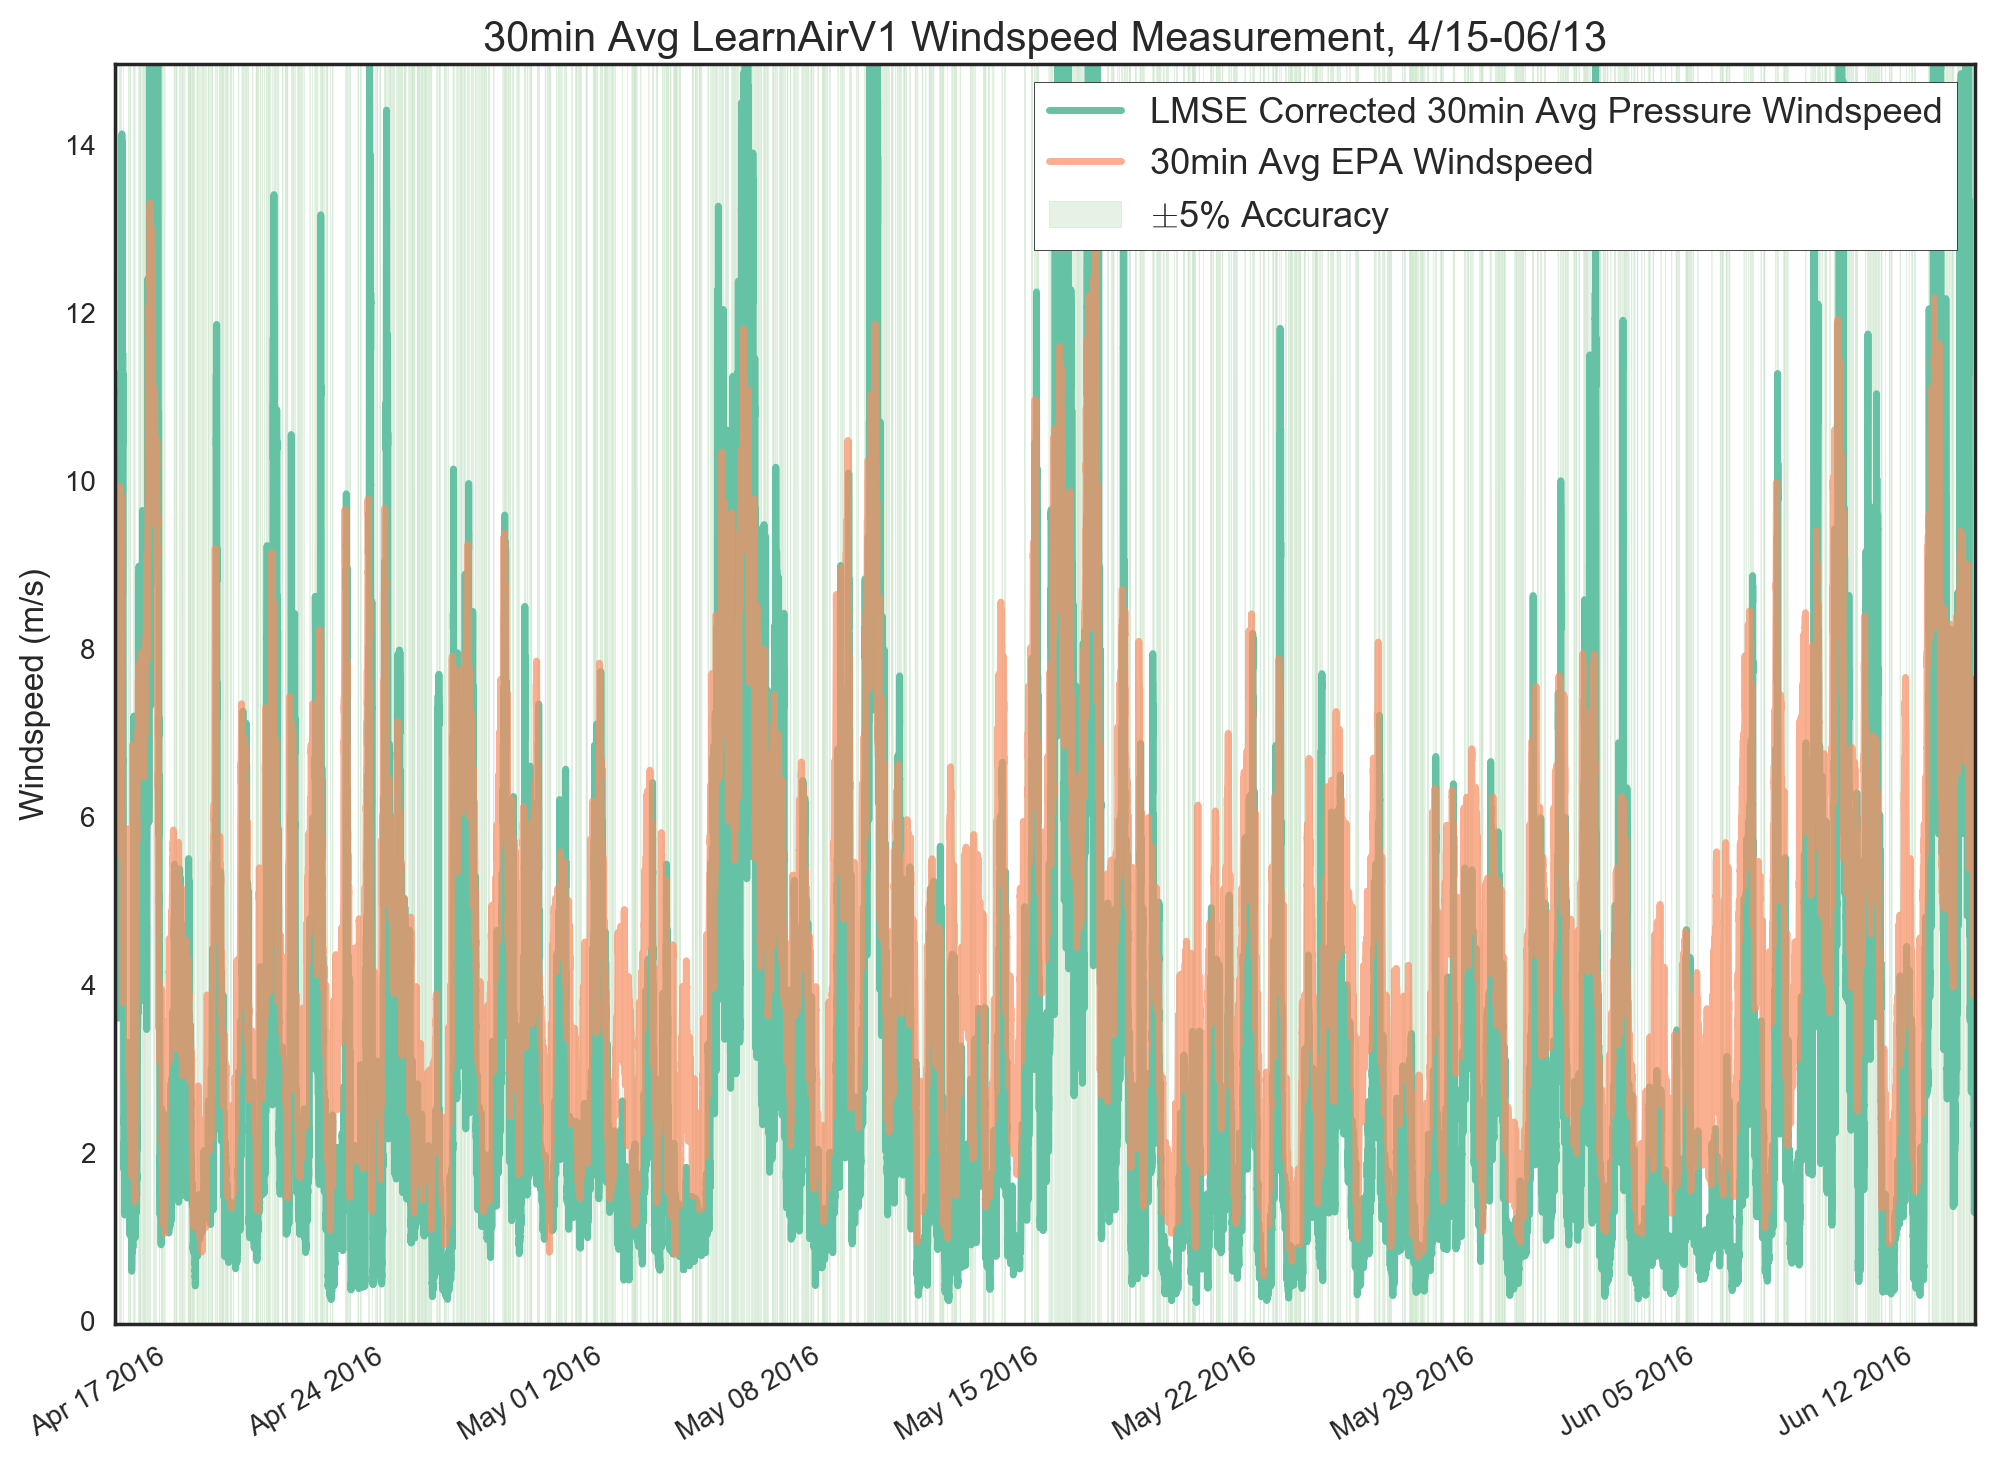
\includegraphics[width=\textwidth]{figs/ws_with_10_accuracy}               
 	 \caption{Wind Speed Measurement with 10\% Accuracy}
  	\label{fig:ws_with_10_accuracy}
\end{figure}

Figure {\ref{fig:wd_with_10_accuracy_zoomed} shows the wind direction angle over the course of a day, with an indication of how closely the conditioned wind pressure sensor reading matched the actual windspeed.  Green highlighting indicates that our windspeed measurement was within $\pm$5\% of the MassDEP reading.  This plot is useful to look for systemic errors-- are there any wind directions where we consistently are accurate in our measurment?  Are there any wind directions where we're inaccurate?  It appears there are no obvious relationships between wind direction and accuracy from this graph.  However, there are interesting relationships between wind direction and error-- please see Chapter 5.
 
\begin{figure}[htb]
 	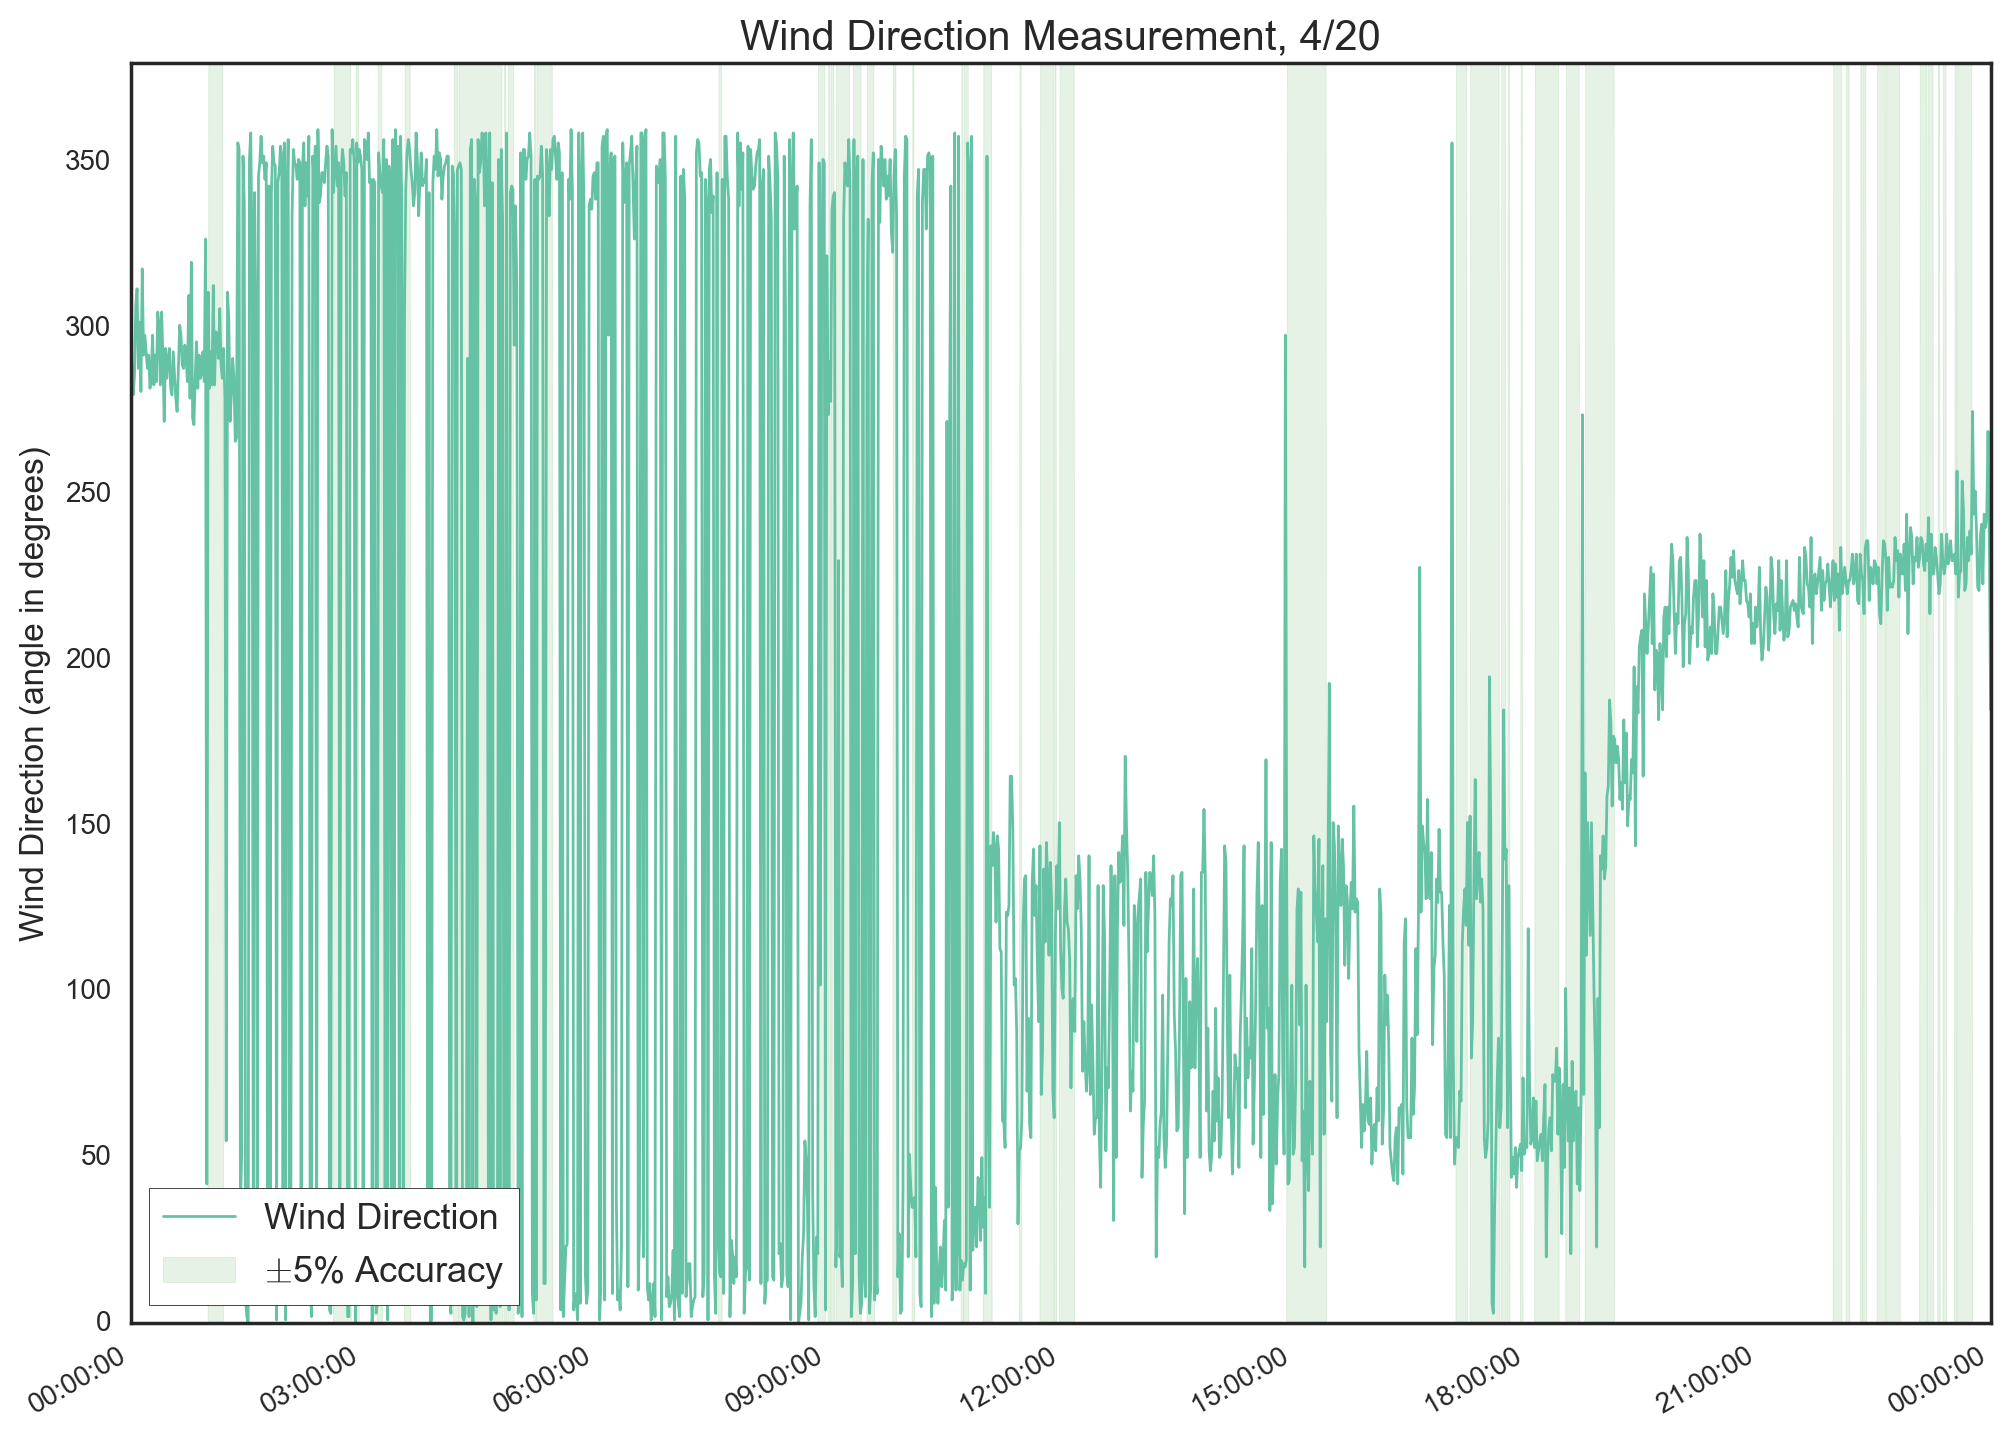
\includegraphics[width=\textwidth]{figs/wd_with_10_accuracy_zoomed}               
 	 \caption{Wind Direction with 10\% Accuracy WindSpeed Measurements Denoted}
  	\label{fig:wd_with_10_accuracy_zoomed}
\end{figure}

\clearpage
\newpage
